\documentclass[10pt]{scrartcl}
\usepackage[pretty]{mystd}
\title{}
\author{}
\date{}

\begin{document}
    %\maketitle
    \subsection*{Morgan Laurent*}
    \begin{exo}[Compacts d'un espace de suites]
        On considère l'ensemble $E\subset \R^{\N}$ constitué des suites réelles bornées, qui est un $\R$-espace vectoriel.
        Pour une suite $u\in E$, on définit $\norm{u}=\sum_{n=0}^{+\infty}|u_n|2^{-n}$. Vérifier que $\norm{\cdot}$ définit une norme sur $E$ 
        et montrer que la partie $A=\lbrace u\in E,\ \forall n\in\N,\ u_n\in[0,1]\rbrace$ est compacte.
    \end{exo}

    \begin{exo}[Norme sur les polynômes]
        On munit $\R[X]$ de la norme $\norm{\cdot}_{\infty}$ définie par $\norm{\sum_{k=0}^{+\infty}a_kX^k}=\text{max}\lbrace |a_k|,\ k\in\N\rbrace$.
        \begin{enumerate}
            \item Montrer que $\mathcal U$ l'ensemble des polynômes unitaires de $\R[X]$ est fermé.
            \item Soit $Q\in\mathcal U$ non constant, on note $p=\deg Q$. Montrer que 
            \[Q\text{ est scindé sur }\R\iff \forall z\in\C,\ |Q(z)|\geq |\Ims(z)|^p\]
            \item Montrer que $\mathcal S$, l'ensemble des polynômes unitaires et scindés de $\R[X]$ est un fermé.
        \end{enumerate}
    \end{exo}

    \begin{exo}[Valeurs d'adhérence]
        \hfill
        \begin{enumerate}
            \item Soit $(E,\norm{\cdot})$ un espace vectoriel normé et $(u_n)$ une suite à valeurs dans $E$.
            On note $\Adh(u)$ l'ensemble des valeurs d'adhérence de la suite $(u_n)$. Montrer que l'on a l'égalité 
            \[
                \Adh(u)=\bigcap_{n\in\N}\overline{\lbrace u_p,\ p\geq n\rbrace}
            \]
            \item Existe-t-il une suite à valeurs dans $\R$ dont l'ensemble des valeurs d'adhérence est $\R$ tout entier ?
        \end{enumerate}
    \end{exo}

    \begin{exo}[Ouvert ? Fermé ? Compact ? Borné ?]
        Soit $E$ l'espace des suites $a\in\R^{\N}$ telles que $\sum a_n$ converge absolument. 
        On munit $E$ de la norme $\norm{a}_\infty=\sup\lbrace |a_n|,\ n\in\N\rbrace$.
        On considère $F$ l'ensemble des suites $a\in E$ telles que 
        \[
            \sum_{n=0}^{+\infty}|a_n|=1
        \]
        Cet ensemble est-il ouvert ? Fermé ? Compact ? Borné ?
    \end{exo}

    \begin{exo}[Espace de fonctions lipschitziennes]
        Soit $E$ l'ensemble des fonctions lipschitziennes de $[0,1]$ dans $\R$.
        \begin{enumerate}
            \item Montrer que $E$ est un espace vectoriel sur $\R$. 
            \item Pour $f\in E$, on note $K(f)$ la plus petite constante de Lipschitz pour $f$. Cette application définit-elle une norme sur $E$ ?
            \item Montrer que $N(f)=K(f)+|f(0)|$ définit une norme sur $E$. Est-elle équivalente à la norme $\norm{\cdot}_\infty$ ?
        \end{enumerate}
    \end{exo}

    \begin{exo}[Encore des normes sur les polynômes]
        Sur l'espace $E=\R[X]$ des polynômes à coefficients réels, on définit 
        \[
            N_1(P)=\sum_{n\geq 0}\left|\frac{P^{(n)}(0)}{n!}\right|\quad N_2(P)=\sup_{n\geq 0}\left|\frac{P^{(n)}(0)}{n!}\right|\quad N_3(P)=\sup_{x\in[0,1]}|P(x)|
        \]
        Vérifier que les $N_i$ sont des normes et qu'elles sont deux à deux non-équivalentes.
    \end{exo}

    \newpage
    \subsection*{Etienne Debacq*}
    \begin{exo}[Norme et convexité]
        Une partie $X$ d'un espace vectoriel $E$ est dite convexe si la condition suivante est vérifiée : 
        \begin{itemize}
            \item[(C1)] $\forall x,y\in X$, $\forall t\in[0,1]$, $tx+(1-t)y\in X$.
        \end{itemize}
        Rappeler la définition d'une norme et montrer que la condition de l'inégalité triangulaire peut être remplacée par :
        \begin{itemize}
            \item[(N1)] L'ensemble $\lbrace x\in E,\ \norm{x}\leq 1\rbrace$ est convexe.
        \end{itemize}

    \end{exo}
    \begin{exo}[Jauge !] Soit $E$ un espace vectoriel de dimension finie sur $\R$.
        \begin{enumerate}
            \item Montrer que la boule unité fermée d'une norme est un compact convexe, symétrique par rapport à $0$ et un voisinage de $0$.
            \item Inversement, soit $K$ un compact convexe de $E$, symétrique par rapport à $0$ et voisinage de $0$. Montrer que $K$ est la boule unité fermée d'une certaine norme sur $E$.
        \end{enumerate}
    \end{exo}

    \begin{exo}[Un exercice sur les compacts]
        Soit $f:\R\to\R$ continue. Montrer l'équivalence de :
        \begin{enumerate}[(i)]
            \item Pour tout compact $K$, $f^{-1}(K)$ est compact ;
            \item $\lim_{x\to \pm\infty}|f(x)|=+\infty$.
        \end{enumerate}
    \end{exo}

    \begin{exo}[Normes sur les fonctions continues]
        On considère $E=\mathcal C^0([0,1],\R)$ et $\rho\in E$ positive ou nulle. Pour toute application $f\in E$, on pose 
        \[
            N_\rho(f)=\int_0^1\rho|f|
        \]
        \begin{enumerate}
            \item Déterminer une CNS sur $\rho$ pour que $N_\rho$ soit une norme sur $E$.
            \item Déterminer une CNS pour que les normes $N_{\rho_1}$ et $\norm{\cdot}_1$ soient équivalentes.
        \end{enumerate}
    \end{exo}

    \begin{exo}
        Soit $P\in\R[X]$. Construire une norme sur $\R[X]$ telle que $(X^n)$ converge vers $P$ pour cette norme.
    \end{exo}

    \begin{exo}
        Montrer que l'ensemble des polynômes de $\C_n[X]$ de degré $n$ admettant $n$ racines simples est un ouvert de $\C_n[X]$.
    \end{exo}

    \begin{exo}
        Montrer que l'ensemble des polynômes de $\R_n[X]$ de degré $n$ scindés à racines simples réelles est une partie ouverte de $\R_n[X]$.
    \end{exo}

    \vspace{2em}
    \begin{center}
        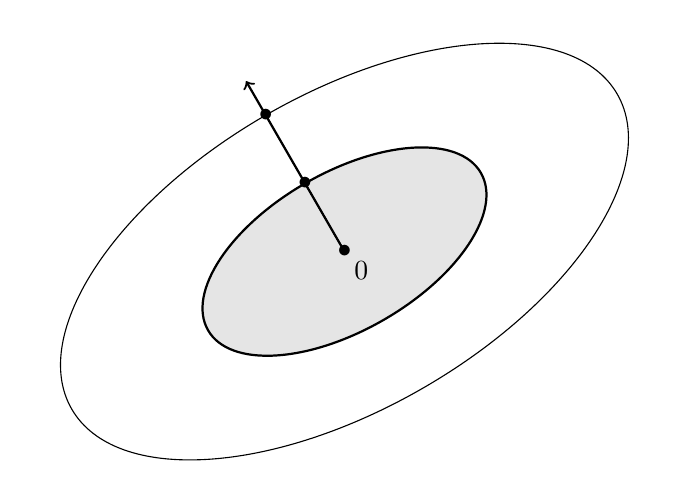
\begin{tikzpicture}
            \fill[fill=gray!20,draw=black,thick] (0,0) circle [x radius=2cm, y radius=10mm, rotate=30];
            \draw[draw=black] (0,0) circle [x radius=4cm, y radius=20mm, rotate=30];
            \node (a) at (0,0) [] {$\bullet$};
            \node (b) at (0,0) [below right] {$0$};
            \draw[rotate=30,thick,->] (0,0) -- ++(0,2.5);
            \draw[rotate=30] (0,0) -- ++(0,2) node [] {$\bullet$};
            \draw[rotate=30] (0,0) -- ++(0,1) node [] {$\bullet$};
        \end{tikzpicture}\\
        \vspace{10pt}
        \textsc{Figure} – \textit{Jauge !}
    \end{center}

    \newpage
    \subsection*{Florian Laffont*}
    \begin{exo}[Adhérence d'un graphe]
        Soit $f:\Rpe\to\R$ l'application définie par $f(x)=\cos(1/x)$. 
        On pose $A=\lbrace (x,f(x)),\ x>0\rbrace\subset\R^2$. Déterminer l'adhérence de $A$.
    \end{exo}

    \begin{exo}[Normes sur les polynômes]
        On considère $E=\R[X]$ l'espace des polynômes à coefficients réels. À toute suite $\lambda$ de réels strictement positifs, on associe $N_\lambda(P)=\sum_{n\geq 0}\lambda_n|{P^{(n)}(0)}|/{n!}$.

        Soient $\lambda$ et $\mu$ deux suites de réels strictements positifs. 
        Après avoir vérifié qu'il s'agit de normes sur $E$, montrer que $N_\lambda$ et $N_\mu$ sont équivalentes si et seulement si les suites $(\lambda_n/\mu_n)$ et $(\mu_n/\lambda_n)$ sont bornées.
    \end{exo}

    \begin{exo}[Condition suffisante de dénombrabilité]
        Soit $A$ une partie de $\R$. 

        Un point $x\in \R$ est dit d'accumulation de $A$ si tout voisinage de $x$ dans $\R$ privé de $x$ rencontre $A$. 
        Montrer que si $A$ est bornée et n'admet qu'un seul point d'accumulation, alors il existe une bijection entre $\N$ et $A$.
    \end{exo}

    \begin{exo}[Normes $p$ sur les espaces de dimension finie]
        On considère $E=\R^n$. On définit les normes suivantes sur $E$ 
        \[
            \norm{x}_p=\left(\sum_{k=1}^n|x_k|^p\right)^{1/p}\quad \norm{x}_\infty=\max_{1\leq k\leq n}|x_k|
        \]
        où $p$ designe un réel plus grand que $1$.

        Pour $p,q\in[1,\infty]$, on note $C_{p,q}$ la plus petite constante telle que 
        \[
            \forall x\in E,\ \norm{x}_q\leq C_{p,q}\norm{x}_p
        \]
        \begin{enumerate}
            \item Justifier l'existence de $C_{p,q}$.
            \item Déterminer $C_{\infty,p}$ et $C_{p,\infty}$ pour $p\in[1,\infty]$.
            \item Montrer que $C_{p,q}=1$ pour $1\leq p\leq q<\infty$. 
            \item Montrer que pour $1\leq q\leq p<\infty$ 
            \[
                C_{p,q}=n^{\frac1q-\frac1p}
            \]
            \textit{Indication : utliser la convexité de l'application $t\mapsto t^{p/q}$ sur $\R_+$}
        \end{enumerate}
    \end{exo}

    \begin{exo}[Intersection d'ouverts denses]
        Soient $U$ et $V$ des ouverts denses d'un espace vectoriel normé $(E,\norm{\cdot})$. 
        Montrer que $U\cap V$ est encore un ouvert dense de $E$.
    \end{exo}

    \begin{exo}[Intersection d'une suite décroissante de compacts non vides]
        Soit $(E,\norm{\cdot})$ un espace vectoriel normé, $(K_n)$ une suite décroissante de compacts non vides de $E$.
        Montrer que $\bigcap_{n\in\N}K_n$ est non vide.
    \end{exo}

    \newpage
    \subsection*{Ronan Kaing}
    \begin{ccp}
        \hfill
        \begin{enumerate}
            \item Rappeler la définition par les suites de vecteurs d'une partie compacte d'un espace vectoriel normé.
            \item Démontrer qu'une partie compacte d'un espace vectoriel normé est une partie fermée de cet espace.
            \item Démontrer qu'une partie compacte d'un espace vectoriel normé est une partie bornée de cet espace.
            \item On se place dans $E=\R[X]$ muni de la norme $\norm{\cdot}_1$ définie pour tout polynôme $P=a_0+a_1X+\dots+a_nX^n$ de $E$ par $\norm{P}_1=\sum_{i=0}^n|a_i|$.
            \begin{enumerate}
                \item Justifier que $S=\lbrace P\in E,\ \norm{P}_1=1\rbrace$ est une partie fermée et bornée de $E$.
                \item Calculer $\norm{X^m-X^n}_1$ pour $m$ et $n$ des entiers distincts. $S$ est-elle une partie compacte de $E$ ? Justifier.
            \end{enumerate}
        \end{enumerate}
    \end{ccp}

    \begin{exo}
        Soient $a_1,\dots,a_n$ des réels et $N:\R^n\to\R$ définie par 
        \[
            N(x_1,\dots,x_n)=a_1|x_1|+\dots+a_n|x_n|
        \]
        Donner une CNS portant sur les $a_k$ pour que $N$ soit une norme sur $\R^n$.
    \end{exo}

    \begin{exo}
        Montrer que si deux boules fermées d'un espace vectoriel normé non nul sont égales, alors elles ont même centre et même rayon.
    \end{exo}

    \begin{exo}
        Démontrer que l'adhérence et l'intérieur d'un convexe d'un espace vectoriel normé sont encore convexes.
    \end{exo}

    \subsection*{Leo Monge}
    \begin{ccp}
        On note $E=\mathcal C^0([0,1],\R)$. 
        On pose pour toute fonction $f\in E$ 
        \[
            N_\infty(f)=\sup_{x\in[0,1]}|f(x)|\quad N_1(f)=\int_0^1|f(t)|\dd t
        \]
        \begin{enumerate}
            \item
            \begin{enumerate}
                \item Démontrer que $N_\infty$ et $N_1$ sont deux normes sur $E$. 
                \item Démontrer qu'il existe $k>0$ tel que $N_1\leq kN_\infty$.
                \item Démontrer que tout ouvert pour la norme $N_1$ est un ouvert pour la norme $N_\infty$.
            \end{enumerate}
            \item Démontrer que les normes $N_1$ et $N_\infty$ ne sont pas équivalentes.
        \end{enumerate}
    \end{ccp}

    \begin{exo}
        Soit $(E_i,\norm{\cdot}_{E_i})_{1\leq i\leq n}$ une famille d'espaces vectoriels normés. 
        On pose $N(x_1,\dots,x_n)=\max_{1\leq i\leq n}\norm{x_i}_{E_i}$ définie sur $E=E_1\times\dots\times E_n$. 
        Montrer que $N$ est une norme sur $E$.
    \end{exo}

    \begin{exo}
        Soient $a,b>0$. On pose pour tout $(x,y)\in\R^2$, $N(x,y)=\sqrt{a^2x^2+b^2y^2}$. 
        \begin{enumerate}
            \item Prouver que $N$ est une norme sur $\R^2$.
            \item Dessiner la boule de centre $0$ et de rayon $1$ pour $N$.
            \item Déterminer le plus petit réel $p>0$ tel que $N\leq p\norm{\cdot}_2$ et le plus grand réel $q>0$ tel que $q\norm{\cdot}_2\leq N$.
        \end{enumerate}
    \end{exo}

    \begin{exo}
        Soit $(u_n)$ une suite de réels.
        \begin{enumerate}
            \item Montrer que si $(u_{2n})$ et $(u_{2n+1})$ convergent vers la même limite, alors $(u_n)$ converge. 
            \item Trouver une suite $(u_n)$ telle que $(u_{2n})$ et $(u_{2n+1})$ convergent, mais pas $(u_n)$.
            \item Montrer que si $(u_{2n})$, $(u_{2n+1})$ et $(u_{3n})$ convergent, alors $(u_n)$ converge.
        \end{enumerate}
    \end{exo}

    \newpage
    \subsection*{Jaufret Patou-Stefaniak}
    \begin{ccp}
        Soit $(E,\norm{\cdot})$ un espace vectoriel normé. Soient $A$ et $B$ deux parties non vides de $E$.
        \begin{enumerate}
            \item 
            \begin{enumerate}
                \item Rappeler la caractérisation de l'adhérence d'un ensemble à l'aide des suites.
                \item Montrer que $A\subseteq B\implies \overline A\subseteq\overline B$.
            \end{enumerate}
            \item Montrer que $\overline{A\cup B}=\overline A\cup\overline B$.
            \item 
            \begin{enumerate}
                \item Montrer que $\overline{A\cap B}\subseteq \overline A\cap\overline B$.
                \item Montrer, à l'aide d'un exemple, que l'autre inclusion n'est pas forcément vérifiée (on prendra $E=\R$).
            \end{enumerate}
        \end{enumerate}
    \end{ccp}

    \begin{exo}
        Soit $(E,\norm{\cdot})$ un espace vectoriel normé et $f:E\to E$ un endomorphisme. 
        Pour $x\in E$, on pose $N(x)=\norm{f(x)}$. 
        Donner une CNS sur $f$ pour que $N$ soit une norme sur $E$.
    \end{exo}

    \begin{exo}
        On considère $E=\mathcal C^0([0,1],\R)$. On définit sur $E$
        \[
            \norm{f}_\infty=\sup_{x\in[0,1]}|f(x)|\quad \norm{f}_1=\int_0^1|f(t)|\dd t
        \]
        On note $F$ l'ensemble des fonctions de $E$ nulles en $0$. 
        Déterminer l'adhérence de $F$ dans $E$ pour les deux normes précédentes.
    \end{exo}

    \begin{exo}
        Soit $(E,\norm{\cdot})$ un espace vectoriel normé.
        \begin{enumerate}
            \item Soient $A$ et $B$ deux parties disjointes de $E$ et on suppose $A$ ouverte. Montrer que $A\cap\overline B=\varnothing$.
            \item Soit $U$ un ouvert non vide. Montrer que $\Vect U=E$.
            \item Quelles sont les parties $A$ de $E$ vérifiant $\Fr(A)=\varnothing$ ?
        \end{enumerate}
    \end{exo}
\end{document}